% !TEX root = ../main.tex

\section{Results}

% \begin{itemize}
%     \item Methods on how we're doing simulations and results (with simulations and experimental data)
%     \begin{itemize}
%         \item Different SNRs and maybe even use CAPs
%         \item Selection of HRF explained if both use the same but it's different from what's used for simulating.
%         \begin{itemize}
%             \item What happens? For example with gamma for simulating.
%         \end{itemize}
%         \item Selection of regularization parameter
%         \begin{itemize}
%             \item Present with real data on a voxel
%         \end{itemize}
%     \end{itemize}
% \end{itemize}

\subsection{Performance based on the regularization parameter}
\label{sec:regpath}

Figure~\ref{fig:sim}A (left) shows the regularization paths of PFM and TA side by side for the three SNR conditions for the spike model; i.e., the inverse problem described in~\eqref{eq:pfm_spike}. Each iteration of LARS reduces the value of \(\lambda\); i.e., reduces the sparsity promoted by the \(l_1\)-norm, and reveals new non-zero coefficients as shown in the x-axis of the heatmaps. Vertical black lines depict the selection of the regularization parameter based on BIC, and thus, the colored coefficients indicated by the vertical lines depict the estimated activity-inducing signal \(s(t)\). Figure~\ref{fig:sim}A (right) illustrates the resulting estimation of the activity-inducing and neuronal-related signals when basing the selection of \(\lambda\) on BIC for the three simulated SNR conditions. Given that the regularization paths of both techniques are identical, the BIC-based selection of the regularization parameter and the results of deconvolving with said \(\lambda\) are identical too. Thus, Figure~\ref{fig:sim}A demonstrates that, regardless of the simulated SNR condition, both deconvolution algorithms produce identical regularization paths when the same HRF and regularization parameters are applied, and hence, identical estimates of the activity-inducing signal \(\mathbf{s}\) and neuronal-related signal \(\mathbf{x}\).

The regularization path to estimate innovation signals yields mainly undistinguishable results for both PFM and TA methods as shown in Figure~\ref{fig:sim}A (left). Again, the BIC-based selection of \(\lambda\) is identical for both PFM and TA, and the estimation of the innovation signal \(\mathbf{u}\) shows no distinguishable differences between the algorithms (see Figure~\ref{fig:sim}A right). Therefore, both PFM and TA yield nearly identical regularization paths and estimates of the innovation signal regardless of the simulated SNR condition when applying the same HRF and regularization parameters with the block model.

% Furthermore, we performed the same analysis on experimental data as shown in Figure~\ref{fig:exp} (rows 1-2, 4). Row 1 demonstrates that the PFM and TA regularization paths are identical when deconvolving experimental data, regardless of the deconvolution model (spike or block). Even though tiny differences can be seen between the two methods in the BIC selection of \(\lambda\) in row 4, row 2 proves that the results are practically identical, and differences can be disregarded.

\begin{figure*}[t!]
    \begin{center}
        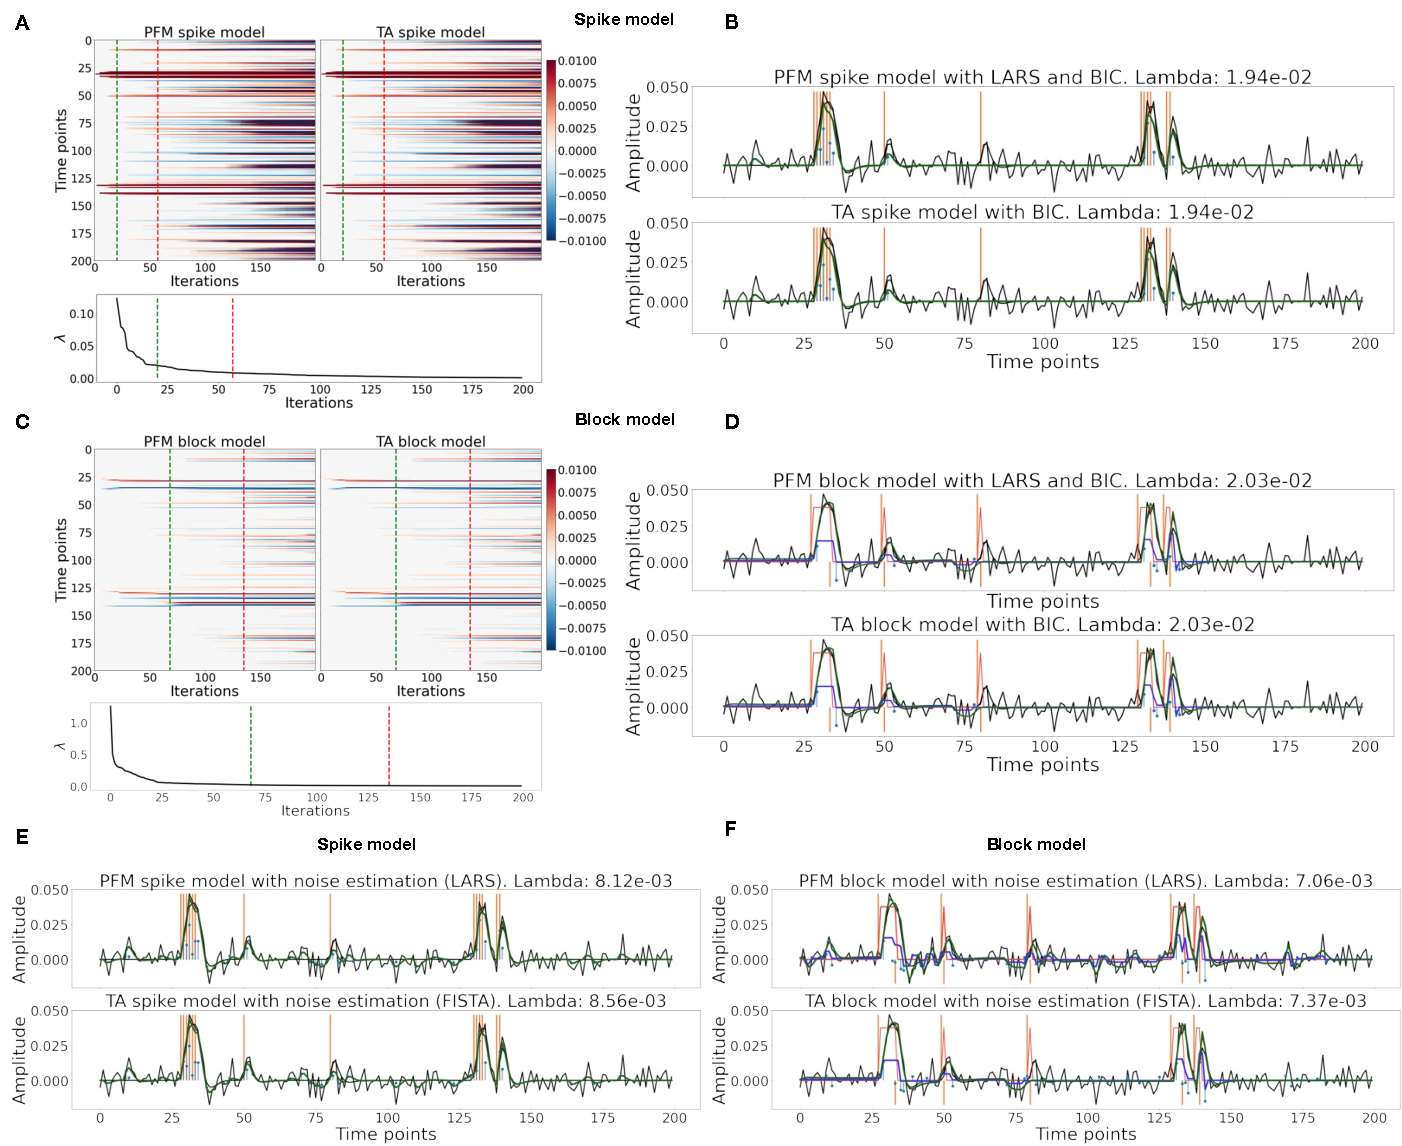
\includegraphics[width=\textwidth]{figures/figure_sim.pdf}
    \end{center}
    \caption{A) (Left) Heatmap of the regularization paths of the activity-inducing (top) and innovation (bottom) signals estimated with PFM and TA as a function of \(\lambda\) for the simulated data with SNR = 3 dB (x-axis: increasing number of iterations or \(\lambda\) as given by LARS; y-axis: time; color: amplitude). Vertical lines denote iterations corresponding to the Akaike and Bayesian Information Criteria (AIC and BIC) optima. (Right) Estimated activity-inducing (blue) and activity-related (green) signals \(\lambda\) is selected based on BIC. B) Estimated activity-inducing, innovation and activity-related (fit, \(\mathbf{x}\)) signals when \(\lambda\) is selected based on the MAD method with the spike model (left, with PFM on the left and TA on the right) and block model (right, with PFM on the left and TA on the right) for the simulated data with SNR = 3 dB.}
\label{fig:sim}
\end{figure*}

% \begin{figure*}[t!]
%     \begin{center}
%         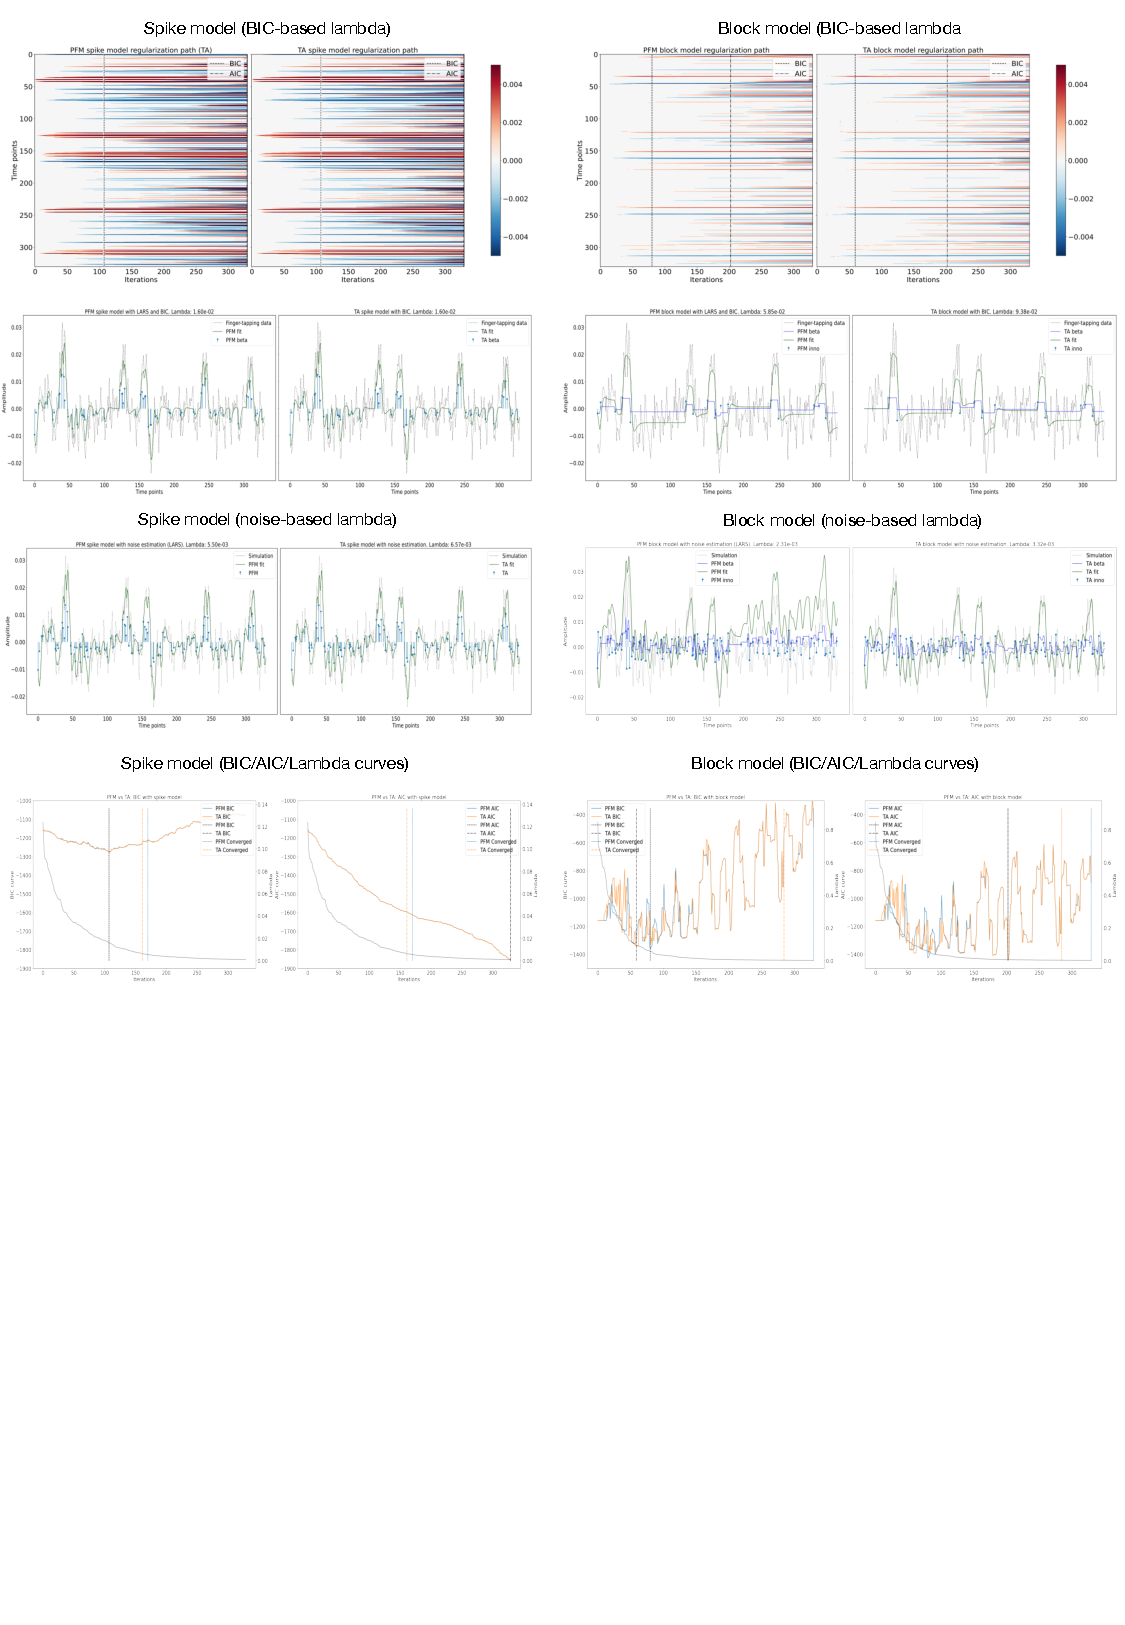
\includegraphics[width=\textwidth]{figures/exp.pdf}
%     \end{center}
%     \caption{(Row 1) Regularization paths of the estimated activity-inducing signal (spike model --- left) and innovation signal (block model --- right); (Row 2) activity-inducing, innovation and activity-related (fit, \(\mathbf{x}\)) signals when \(\lambda\) is selected based on BIC, or (Row 3) based on convergence of residuals to have same variance as MAD estimate of noise; (Row 4) Corresponding cost curves of BIC and AIC. The vertical lines indicate the three options to select \(\lambda\) (BIC, AIC and Converged/MAD).}
% \label{fig:exp}
% \end{figure*}

 Figure~\ref{fig:sim}B depicts the estimated activity-inducing, innovation, and activity-related signals when updating \(\lambda\) following~\eqref{eq:std} in the three simulated SNR settings using the spike model (left) and the block model (right). Figure~\ref{fig:sim}B (left) shows nearly identical results between PFM (left) and TA (right) with the use of the spike model. The minimal differences are the result of slight dissimilarities in the convergence of the residuals to the estimated noise level of the data. Likewise, the use of the block model with a selection of \(\lambda\) based on the MAD estimate of the noise yields results that are identical in practice as shown in Figure~\ref{fig:sim}B (right).

\subsection{Performance on experimental data}

Figure~\ref{fig:rss} depicts the SSD of the spike (Figure~\ref{fig:rss}A) and block (Figure~\ref{fig:rss}B) models for the three experimental datasets introduced: i.e., motor, monoband and multiband. SSD values are clearly lower than those of the activity-inducing and innovation signals, suggesting that the differences between PFM and TA are negligible. The largest differences are evident in regions with high vasculature, likely resulting from differences in amplitude of activity-inducing and innovation signals. \todo{Expand more on interpretation of this Figure.}

\begin{figure*}[t!]
    \begin{center}
        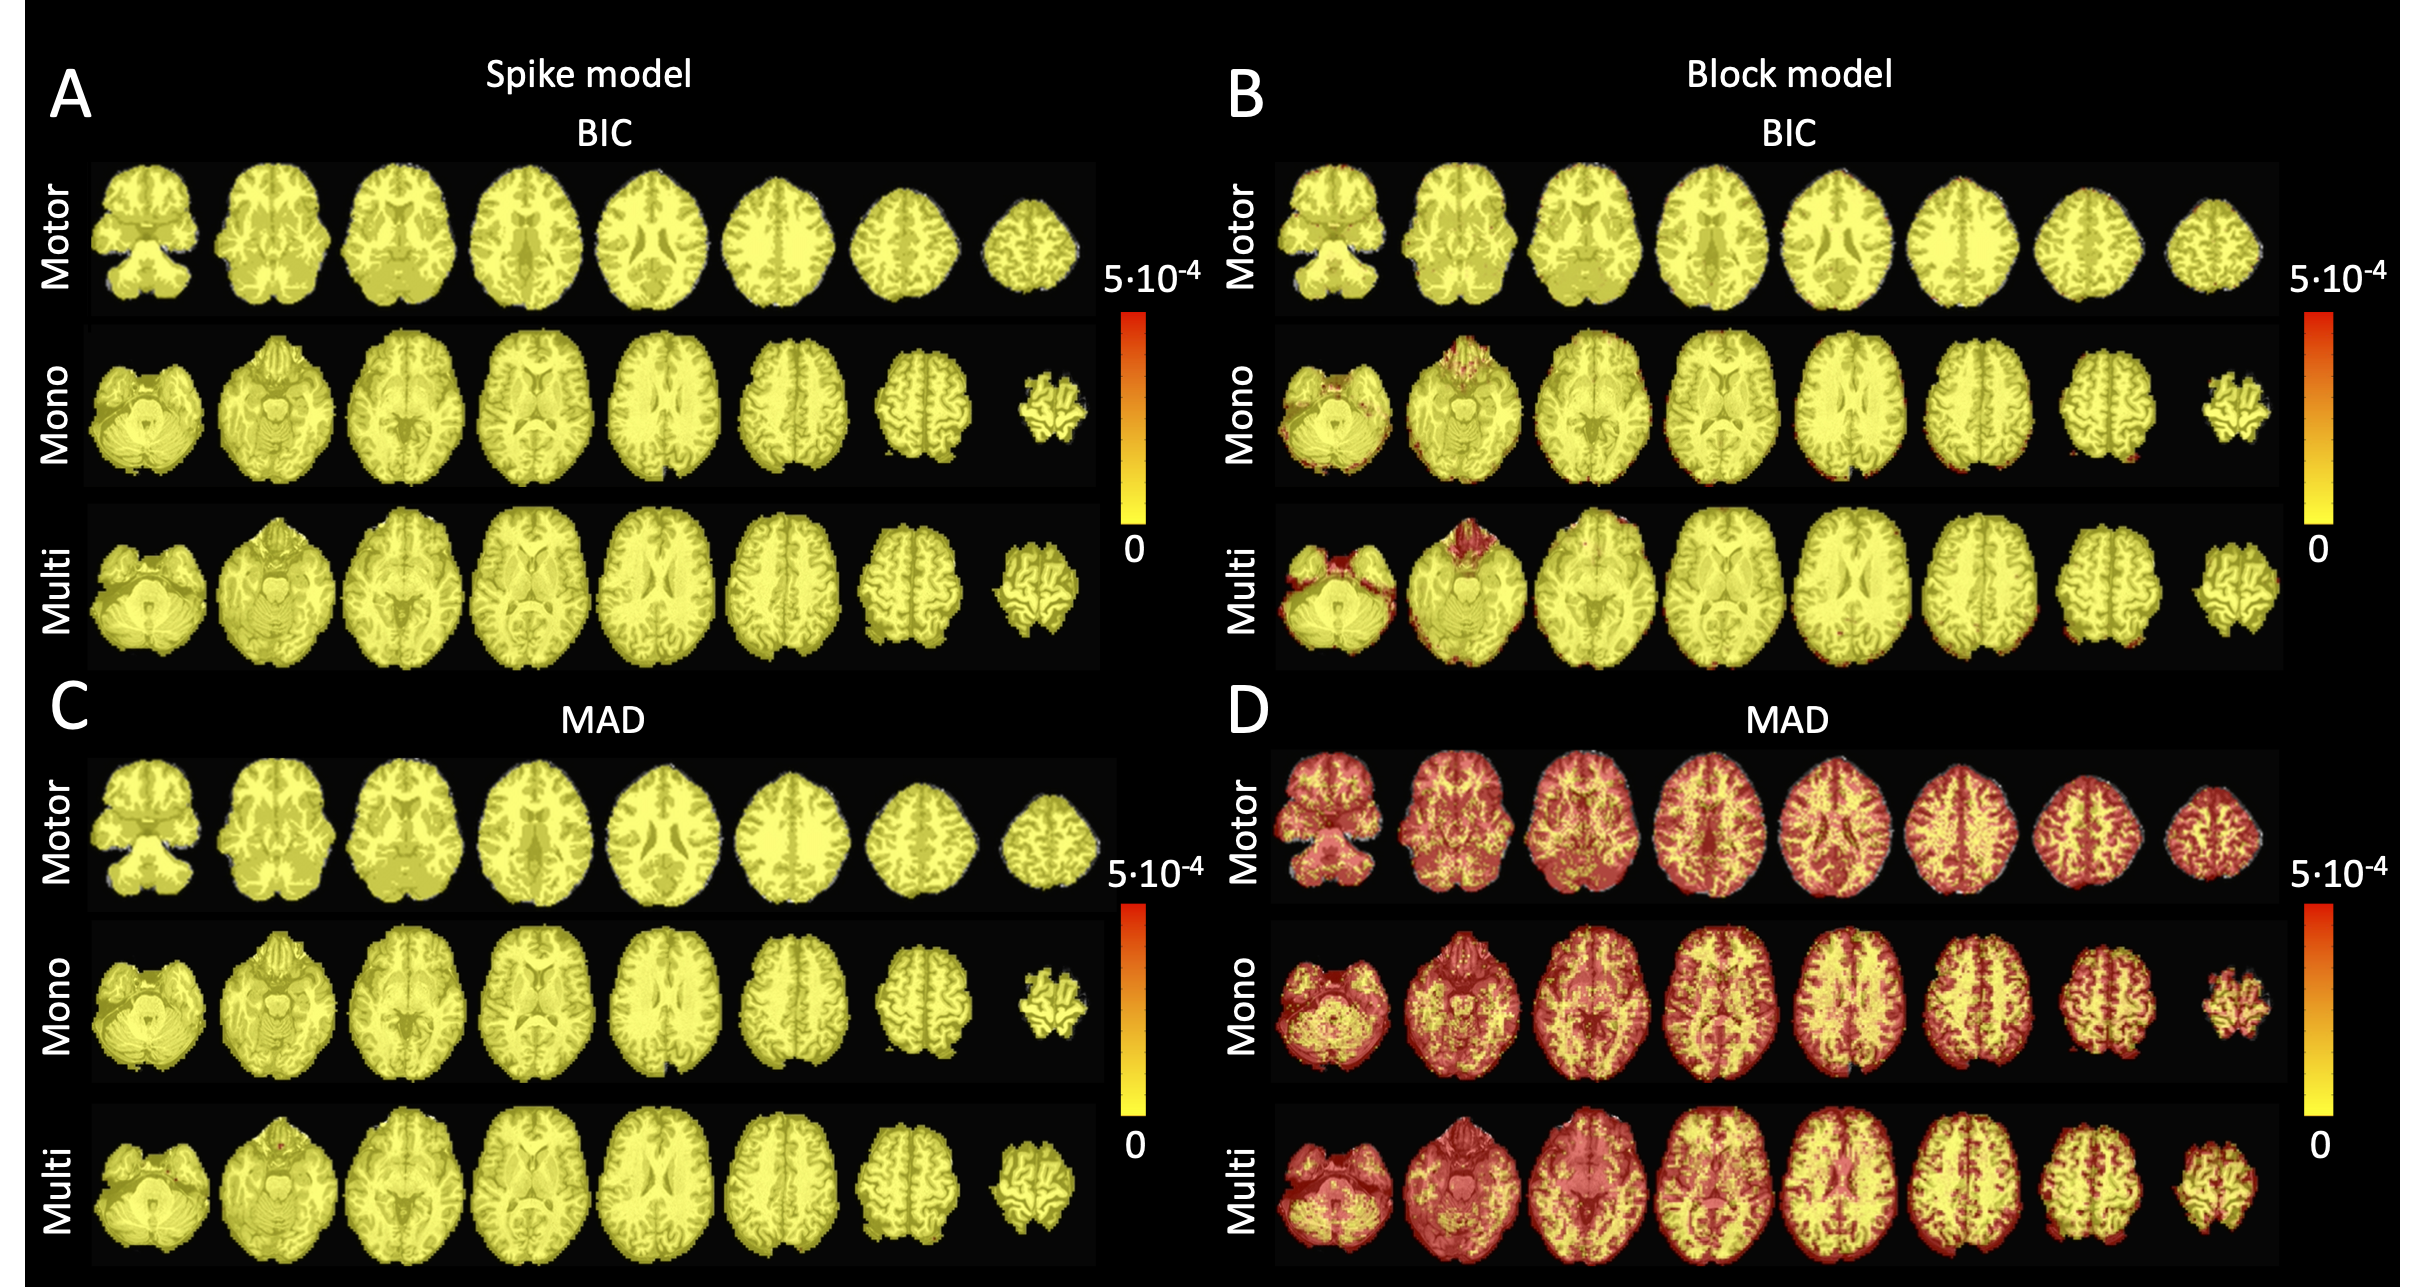
\includegraphics[width=\textwidth]{figures/comp_figure.png}
    \end{center}
    \caption{Sum of squares of the differences of the activity-inducing and innovation signals estimated with Paradigm Free Mapping and Total activation for the different selections of the regularization parameter: BIC (top), and MAD (bottom). The sum of square difference maps are shown for the three experimental datasets introduced in Section~\ref{sec:data}: the motor task (Motor), the monoband resting-state (Mono), and the multiband resting-state (Multi) datasets. A) Sum of squares of the differences when using the spike model. B) Sum of squares of the differences when using the block model.}
\label{fig:rss}
\end{figure*}

Figure~\ref{fig:task_maps} illustrates the activation time-series, activation maps and PFM-estimated (BIC) activity-related, activity-inducing and innovation signals of a representative voxel in the activated region of each of the conditions of the motor task data. The TA-estimated time-series are not shown due to its identical performance. The activation time-series, calculated as the sum of squares of all voxel amplitudes for a given moment in time, of PFM and TA show nearly identical patterns. Furthermore, the estimated activity-related, activity-inducing and innovation signals clearly reveal the activity patterns of each condition in the task, as they exhibit a BOLD response locked to the onset and duration of the conditions. Overall, activity maps of the innovation signal obtained with PFM and TA highly resemble those obtained with GLM for individual events and the differences between PFM and TA can be disregarded as the values are close to zero and do not represent a response to the task.

\begin{figure*}[t!]
    \begin{center}
        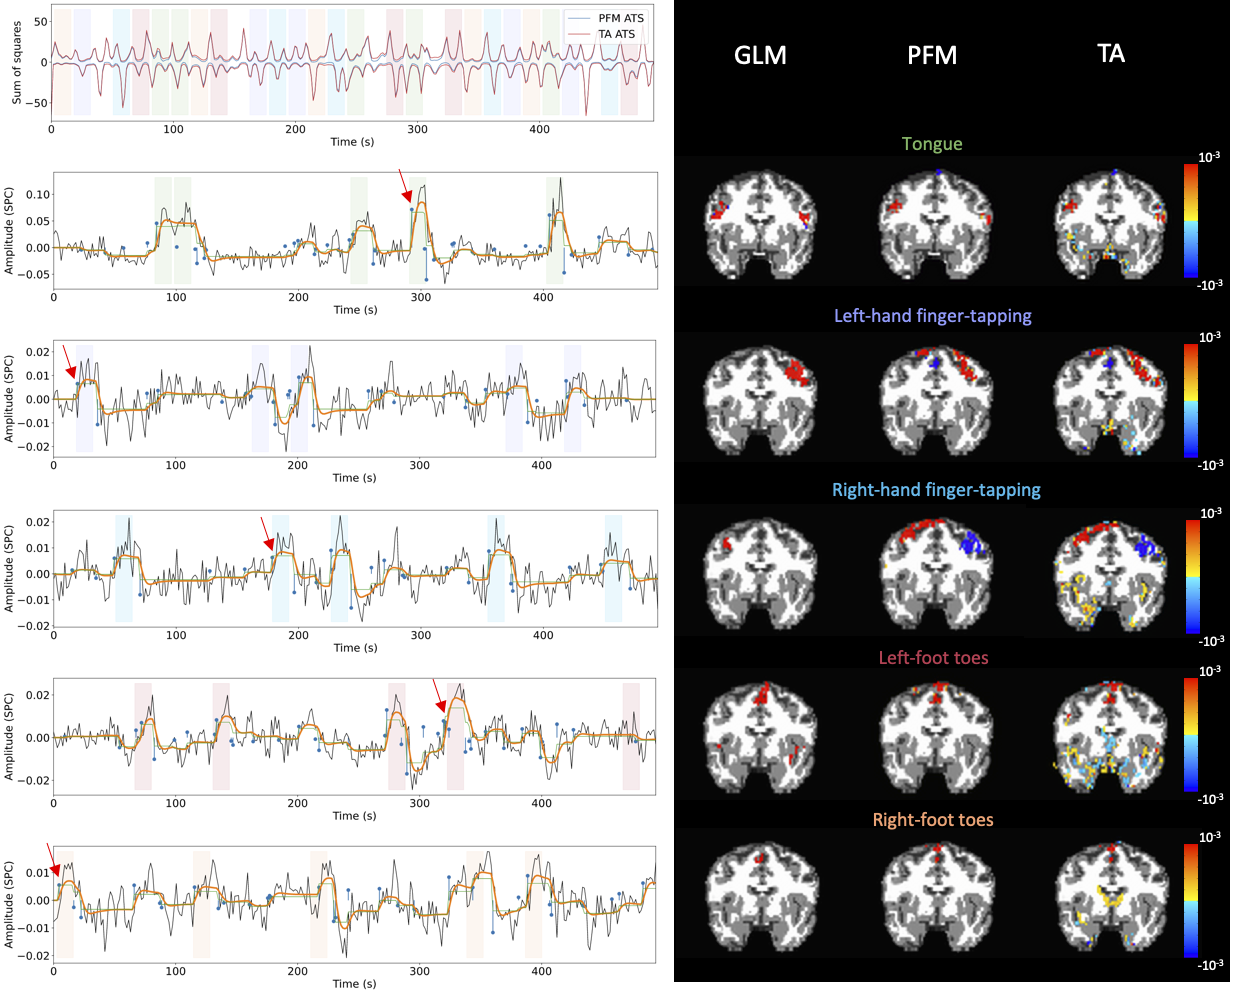
\includegraphics[width=\textwidth]{figures/task_maps.png}
    \end{center}
    \caption{Row 1: Activation time-series of the innovation signals estimated by PFM (in blue) or TA (in red) calculated as the sum of squares at every time-frame. Positive-valued and negative-valued contributions were separated into two distinct time-courses. Color-bands indicate the onset and duration of each condition in the task (green: tongue, purple: left-hand finger-tapping, blue: right-hand finger-tapping, red: left-foot toes, orange: right-foot toes). Rows 2-6: time-series of a representative voxel for each task with the PFM-estimated innovation (blue), PFM-estimated activity-inducing (green), and activity-related (i.e., fitted, orange) signals, with their corresponding GLM, PFM, and TA maps on the right. The maps shown on the right are sampled at the time-point labeled with the red arrows and display the innovation signals at that moment across the whole brain.}
\label{fig:task_maps}
\end{figure*}

\subsection{Co-activation patterns}

Figure~\ref{fig:caps} depicts the CAPs and iCAPs obtained from thresholding and averaging the activity-inducing and innovation signals estimated from the multiband data using PFM. Activity maps obtained with the CAPs method show spatial patterns of the default mode network (DMN), dorsal attention network (DAN) and visual network (VIS) that are cleaner than those obtained from the original data, while mantaining the structure of the networks. On the other hand, spatial patterns acquired with the iCAPs approach, i.e., using the block model, are not as comparable as those obtained with the spike model. 

\begin{figure*}[t!]
    \begin{center}
        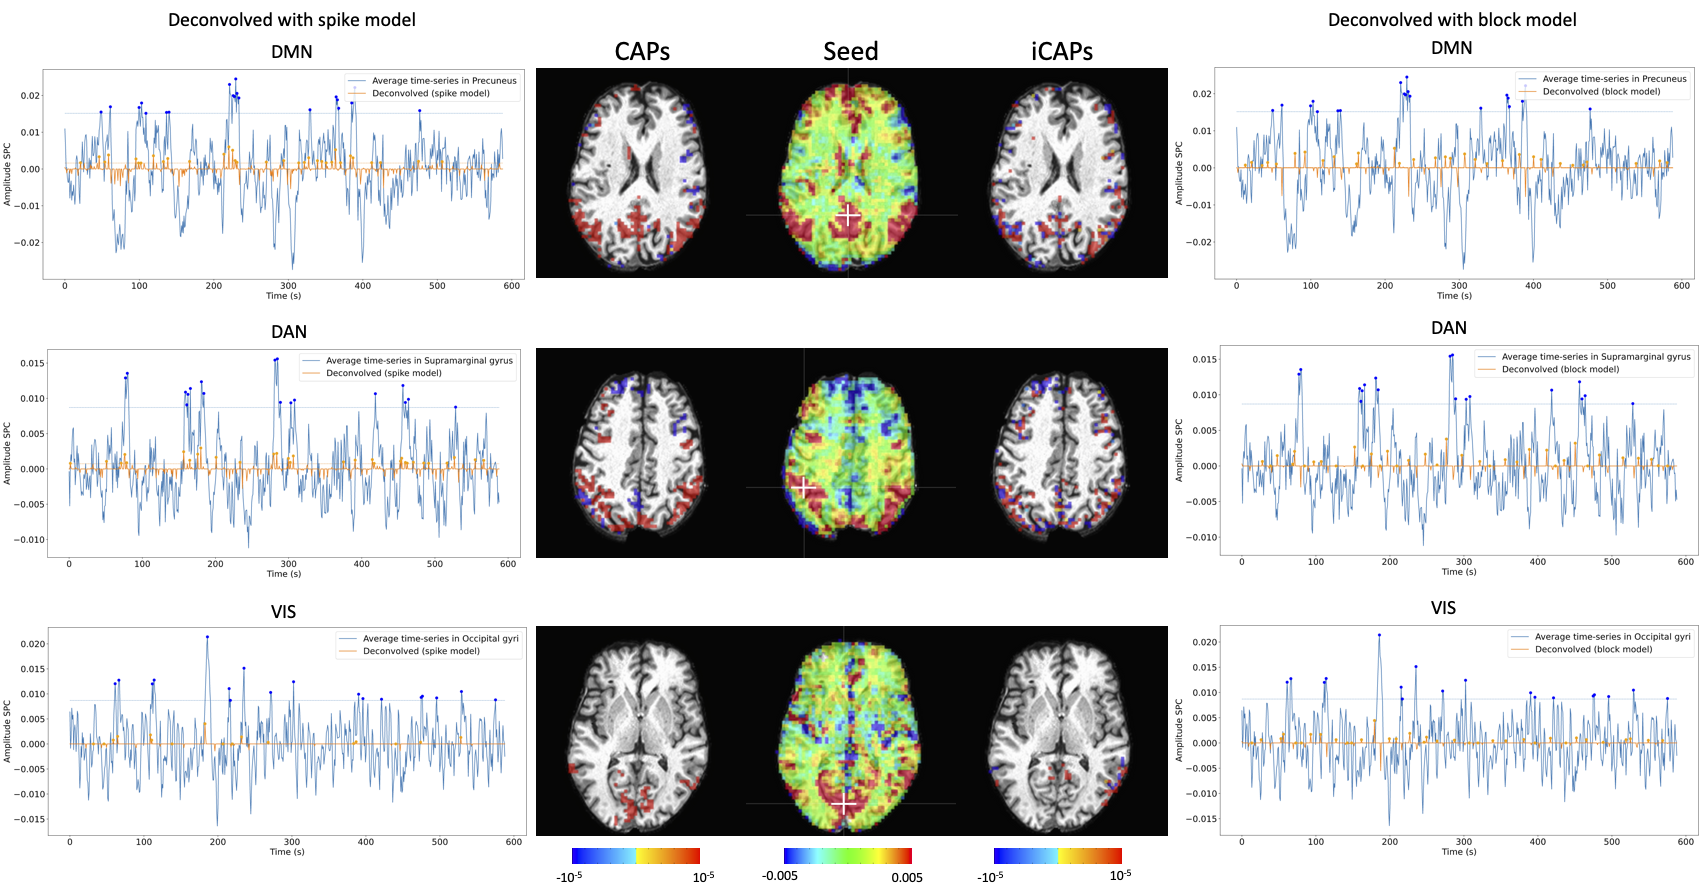
\includegraphics[width=\textwidth]{figures/caps.png}
    \end{center}
    \caption{CAPs (left) and iCAPs (right) obtained with the PFM-estimated activity-inducing and innovation signals, respectively. Time-points selected with a 95th percentile threshold are shown over the average time-series (blue) in the seed region (white-cross) and the deconvolved signal (orange). CAPs and iCAPs maps of the seed and deconvolved signals obtained by averaging the selected time-points are illustrated in the center.}
\label{fig:caps}
\end{figure*}

\todo[inline]{What about computation time? Do something similar as Hamza in his PhD?}
\todo[inline]{What about Figs. 6 and 7? Why is PFM and TA not equivalent there?}